\documentclass{ctexbook}
\input{D:/Repository/Notebook_by_Leo_Yan/note-setup.tex}
\usepackage{wrapfig}
\usepackage{multicol}
\usepackage{paracol}
\usepackage{varwidth}
\usepackage{dsfont}
\usepackage{fix-cm}
\usepackage{array}
\usepackage{booktabs}
\usepackage{float}
\usepackage{pifont}
\usepackage{enumitem}
\usepackage{circuitikz}
\usepackage{tikz}
\usetikzlibrary{arrows.meta, positioning, shapes,calc}
\usepackage{standalone}
\usepackage{silence}
\usetikzlibrary{calc}
\allowdisplaybreaks
\raggedbottom
\usetikzlibrary{shapes,arrows,positioning,calc}
\usepackage{graphicx}
\usepackage{grffile}
\graphicspath{{D:/Repository/Notebook_by_Leo_Yan/Figures/}}
\let\cleardoublepage\clearpage
\usepackage{url}

\title{信息论}
\author{Leo Yan}
\date{\today}

\begin{document}
\maketitle
\tableofcontents
\clearpage
\chapter{熵,相对熵,互信息}

\section{基本概念}

\begin{definition}[熵]
    设X是离散型随机变量,取值(样本空间)为$\mathcal{X}$,概率分布为$p(x)$,则X的熵(entropy)定义为
    \[H(X) = -\sum_{x \in \mathcal{X}} p(x) \log p(x)=\mathbb{E} _p\left[\log \frac{1}{p(X)}\right]\]
    单位为比特(bit);若以自然对数为底,则单位为纳特(nat)
    \[H(X)\geq 0;\quad H_b(X)=\log_b a\cdot H_a(X)\]
    也记为$H(p)$
\end{definition}
\begin{remark}
    熵描述随机变量的不确定度;给出了描述随机变量所需的信息量的下界
\end{remark}

\begin{definition}[联合熵]
    设(X,Y)为联合分布的离散型随机变量,则(X,Y)的联合熵(joint entropy)定义为
    \[H(X,Y) = -\sum_{x \in \mathcal{X}} \sum_{y \in \mathcal{Y}} p(x,y) \log p(x,y)=\mathbb{E} _p\left[\log \frac{1}{p(X,Y)}\right]\]
    也记为$H(XY)$
\end{definition}

\begin{definition}[条件熵]
    设(X,Y)为联合分布的离散型随机变量,则在已知Y的条件下X的条件熵(conditional entropy)定义为
    \[H(X|Y) = -\sum_{y \in \mathcal{Y}} p(y) \sum_{x \in \mathcal{X}} p(x|y) \log p(x|y)=\mathbb{E} _p\left[\log \frac{1}{p(X|Y)}\right]\]
\end{definition}

\begin{theorem}[链式法则]
    设(X,Y)为联合分布的离散型随机变量,则有
    \[H(X,Y) = H(X) + H(Y|X) = H(Y) + H(X|Y)\]
\end{theorem}
\begin{proof}
    \begin{align*}
        H(X,Y) &= -\sum_{x \in \mathcal{X}} \sum_{y \in \mathcal{Y}} p(x,y) \log p(x,y) \\
        &= -\sum_{x \in \mathcal{X}} \sum_{y \in \mathcal{Y}} p(x)p(y|x) \log [p(x)p(y|x)] \\
        &= -\sum_{x \in \mathcal{X}} \sum_{y \in \mathcal{Y}} p(x,y) \log p(x) - \sum_{x \in \mathcal{X}} \sum_{y \in \mathcal{Y}} p(x,y) \log p(y|x) \\
        &= H(X) + H(Y|X)
    \end{align*}
\end{proof}

\begin{definition}[相对熵]
    设p和q为定义在同一样本空间$\mathcal{X}$上的两个离散概率分布,则p相对于q的相对熵(relative entropy)或Kullback-Leibler散度(KL散度)定义为
    \[D(p||q) = \sum_{x \in \mathcal{X}} p(x) \log \frac{p(x)}{q(x)} = \mathbb{E} _p\left[\log \frac{p(X)}{q(X)}\right]\]
\end{definition}
\begin{remark}
    描述两个概率分布之间的差异;真实分布为p,假设分布为q的无效性
\end{remark}

\begin{definition}[互信息]
    设(X,Y)为联合分布的离散型随机变量,则X和Y的互信息(mutual information)定义为
    \[I(X;Y) = D(p(x,y)||p(x)p(y)) = \sum_{x \in \mathcal{X}} \sum_{y \in \mathcal{Y}} p(x,y) \log \frac{p(x,y)}{p(x)p(y)} = \mathbb{E} _p\left[\log \frac{p(X,Y)}{p(X)p(Y)}\right]\]
\end{definition}
\begin{remark}
    描述两个随机变量之间共享的信息量,或X包含Y的信息量
\end{remark}

\begin{proposition}[互信息的性质]
    设(X,Y)为联合分布的离散型随机变量,则有
    \begin{enumerate}
        \item $I(X;Y) = H(X) - H(X|Y) = H(Y) - H(Y|X)$
        \item $I(X;Y) = H(X) + H(Y) - H(X,Y)$
        \item $I(X;X) = H(X)$
    \end{enumerate}
\end{proposition}
\begin{remark}
    以上三条性质的直观:
    \begin{itemize}
        \item 给定X,Y的不确定性减少了$I(X;Y)$
        \item 容斥原理
        \item 熵又是自信息(self-information)
    \end{itemize}
\end{remark}

\section{多维随机变量}

\textbf{符号说明}

(1)$H(X,Y,Z)$实际上应该理解为$H((X,Y,Z))$,即H总为一元函数

(2)$I(X;Y,Z)$实际上应该理解为$I(X;(Y,Z))$,即$I(\cdot;\cdot)$总为二元函数

(3)$H(X,Y|Z)$实际上应该理解为$H((X,Y)|Z)$,即$H(\cdot|\cdot)$总为二元函数;同理$I(X;Y|Z)$实际上应该理解为$I(X;Y|Z)$,即$I(\cdot;\cdot|\cdot)$总为三元函数。应该认为“;”的优先级高于“$|$”

(4)D虽称为熵,但不是随机变量的函数,而是分布的函数。"$\|$"类似于“;”,D总为二元函数

\begin{definition}[条件互信息]
    X,Y在已知Z的条件下的条件互信息(conditional mutual information)定义为
    \[I(X;Y|Z) = \sum_{z \in \mathcal{Z}} p(z) \sum_{x \in \mathcal{X}} \sum_{y \in \mathcal{Y}} p(x,y|z) \log \frac{p(x,y|z)}{p(x|z)p(y|z)} = \mathbb{E} _p\left[\log \frac{p(X,Y|Z)}{p(X|Z)p(Y|Z)}\right]\]
\end{definition}
\begin{remark}
    描述已知Z,给出Y引起的X的不确定度减少量
\end{remark}

\begin{definition}[条件相对熵]
    对于联合概率质量函数$p(x,y)$和$q(x,y)$,X在已知Y的条件下的条件相对熵(conditional relative entropy)定义为
    \[D(p(x|y)||q(x|y)) = \sum_{y \in \mathcal{Y}} p(y) \sum_{x \in \mathcal{X}} p(x|y) \log \frac{p(x|y)}{q(x|y)} = \mathbb{E} _p\left[\log \frac{p(X|Y)}{q(X|Y)}\right]\]
\end{definition}

\begin{theorem}[熵的链式法则]
    \[H(X_1,X_2,\ldots,X_n) = \sum_{i=1}^n H(X_i|X_{1},X_{2},\ldots,X_{i-1})\]
\end{theorem}
\begin{proof}
    反复使用
    \[H(X,Y) = H(X) + H(Y|X)\]
\end{proof}

\begin{theorem}[互信息的链式法则]
    \[I(X;Y_1,Y_2,\ldots,Y_n) = \sum_{i=1}^n I(X;Y_i|Y_{1},Y_{2},\ldots,Y_{i-1})\]
\end{theorem}
\begin{proof}
    \[I(\mathbf{X};\mathbf{Y}) = H(\mathbf{Y}) - H(\mathbf{Y}|\mathbf{X})\]
\end{proof}

\begin{theorem}[相对熵的链式法则]
    \[D(p(x,y)||q(x,y)) = D(p(x)||q(x)) + D(p(y|x)||q(y|x))\]
\end{theorem}
\begin{proof}
    \begin{align*}
        D(p(x,y)||q(x,y)) &= \mathbb{E} _{p(x,y)}\log \frac{p(X,Y)}{q(X,Y)} \\
        &= \mathbb{E} _{p(x,y)}\log \frac{p(X)p(Y|X)}{q(X)q(Y|X)} \\
        &= \mathbb{E} _{p(x)}\log \frac{p(X)}{q(X)} + \mathbb{E} _{p(x,y)}\log \frac{p(Y|X)}{q(Y|X)} \\
        &= D(p(x)||q(x)) + D(p(y|x)||q(y|x))
    \end{align*}
\end{proof}

\section{不等式}

\begin{theorem}[Jensen不等式]
    设X为离散型随机变量,取值(样本空间)为$\mathcal{X}$,概率分布为$p(x)$,且$f$为凸函数,则有
    \[\mathbb{E} _p[f(X)] \geq f(\mathbb{E} _p[X])\]
    进一步,若f为严格凸函数,则等号成立$\iff X=\mathbb{E}X$
\end{theorem}

\begin{theorem}[信息不等式]
    设p和q为定义在同一样本空间$\mathcal{X}$上的两个离散概率分布,则有
    \[D(p||q) \geq 0\]
    取等$\iff p=q$    
\end{theorem}
\begin{proof}
    $\log$在$(0,+\infty)$上为严格凹函数,故$-\log$为严格凸。考虑
    \[A=\{x\in \mathcal{X}: p(x)>0,q(x)>0\}\]
    则由Jensen不等式,
    \begin{align*}
        D(p||q) &= \sum_{x \in A} p(x) \log \frac{p(x)}{q(x)} \\
        &= -\sum_{x \in A} p(x) \left[-\log \frac{q(x)}{p(x)}\right] \\
        &\geq -\log \left(\sum_{x \in A} p(x) \frac{q(x)}{p(x)}\right) \\
        &= -\log \left(\sum_{x \in A} q(x)\right) \\
        &\geq 0
    \end{align*}
\end{proof}
\begin{corollary}
    \[I(X;Y) \geq 0\]
    取等$\iff X$与$Y$独立

    条件相对熵、条件互信息也是非负的
\end{corollary}
\begin{corollary}
    \[H(X|Y) \leq H(X)\]
    取等$\iff X$与$Y$独立
\end{corollary}
\begin{remark}
    条件导致熵减小。但$H(X|Y=y)$可能大于$H(X)$,不等式仅描述平均性质
\end{remark}

\begin{theorem}
    \[H(X) \leq \log |\mathcal{X}|\]
    取等$\iff X\sim U_{\mathcal{X} }$
\end{theorem}
\begin{corollary}[熵的独立界]
    \[H(X_1,X_2,\ldots,X_n) \leq \sum_{i=1}^n H(X_i)\]
    取等$\iff X_1,X_2,\ldots,X_n$相互独立
\end{corollary}
\begin{proof}
    由链式法则,
    \[H(X_1,X_2,\ldots,X_n) = \sum_{i=1}^n H(X_i|X_{1},X_{2},\ldots,X_{i-1}) \leq \sum_{i=1}^n H(X_i)\]
\end{proof}

\section{其他背景下的不等式}

\begin{definition}
    如果Z的条件分布$p(z|x,y)$仅依赖于y而与x条件独立,即
    \[p(x,y,z) = p(x)p(y|x)p(z|y)\]
    则称随机变量三元组(X,Y,Z)构成马尔可夫链(Markov chain),记为$X \to Y \to Z$

    条件独立的意思是
    \[p(x,z|y) = p(x|y)p(z|y)\]
    X,Z对称,即$X \to Y \to Z \iff Z \to Y \to X$,因此可记$X \leftrightarrow Y \leftrightarrow Z$
\end{definition}

\begin{theorem}[数据处理不等式]
    设随机变量三元组(X,Y,Z)构成马尔可夫链$X \to Y \to Z$,则有
    \[I(X;Y) \geq I(X;Z)\]
    取等$\iff X \to Z \to Y$
\end{theorem}
\begin{proof}
    用互信息的链式法则,
    \[I(X;Y,Z) = I(X;Y) + I(X;Z|Y) = I(X;Z) + I(X;Y|Z)\]
    给定Y,X与Z独立,即$I(X;Z|Y)=0$,而$I(X;Y|Z)\geq 0$,故
    \[I(X;Y) \geq I(X;Z)\]
\end{proof}
\begin{remark}
    对Y的数据处理不能增加其包含X的信息
\end{remark}
\begin{corollary}
    \[I(X;Y)\geq I(X,g(Y))\]
    \[X \to Y \to Z\implies I(X;Y|Z)\leq I(X;Y)\]
\end{corollary}
\begin{remark}
    观察下游随机变量,X,Y的依赖程度可能降低
\end{remark}

\begin{definition}[充分统计量]
    假定有一族概率质量函数$\{f_{\theta}(x)\}$,X是从其中一个分布$f_{\theta}(x)$中抽取的样本,T(X)是X的一个统计量,则
    \[\theta \to X \to T(X)\]
    由数据处理不等式,有
    \[I(\theta;X) \geq I(\theta;T(X))\]
    取等时统计量T(X)未损失X关于参数$\theta$的信息,称T(X)为关于分布族$\{f_{\theta}(x)\}$的充分统计量(sufficient statistic)

    等价定义:给定T(X),X与$\theta$条件独立,即$\theta \to T(X) \to X$
\end{definition}

\begin{definition}[最小充分统计量]
    关于分布族$\{f_{\theta}(x)\}$的充分统计量T(X)是其他任何充分统计量$U(X)$的函数,则称T(X)为关于$\{f_{\theta}(x)\}$的最小充分统计量(minimal sufficient statistic)
    
    定义蕴含$\theta \to T(X) \to U(X) \to X$
\end{definition}
\begin{remark}
    最小充分统计量最大程度地压缩了样本X中关于$\theta$的信息,而其他充分统计量可能包含冗余信息
\end{remark}

由随机变量Y估计与之有关的X,X的估计值记为$\hat{X}=g(Y)$取值空间为$\hat{\mathcal{X}}$,则有马尔可夫链$X \to Y \to \hat{X}$。定义误差概率$P_e = P\{\hat{X} \neq X\}$。
\begin{theorem}[Fano不等式]
    设X为离散型随机变量,取值(样本空间)为$\mathcal{X}$,则有
    \[H(P_e) + P_e \log (|\mathcal{X}| - 1) \geq H(X|\hat{X})\geq H(X|Y)\]
    可减弱为
    \[1+P_e \log |\mathcal{X}|\geq H(X|Y)\implies P_e \geq \frac{H(X|Y)-1}{\log |\mathcal{X}|}\]
\end{theorem}
\begin{proof}
    设错误指示变量$E=\mathds{1} _{\{\hat{X} \neq X\}}$,则有马尔可夫链$X \to Y \to \hat{X} \to E$。由链式法则,
    \begin{align*}
        H(X,E|\hat{X}) &= H(E|\hat{X}) + H(X|E,\hat{X}) \\
        &= H(X|\hat{X}) + H(E|X,\hat{X})
    \end{align*}
    因为$H(E|X,\hat{X})=0$,所以
    \[H(X|\hat{X}) = H(E|\hat{X}) + H(X|E,\hat{X})\]
    注意到
    \[H(E|\hat{X}) \leq H(E) = H(P_e)\]
    且
    \[H(X|E,\hat{X}) = P_e H(X|\hat{X},E=1) + (1-P_e)H(X|\hat{X},E=0) \leq P_e \log (|\mathcal{X}| - 1)\]
    故
    \[H(X|\hat{X}) \leq H(P_e) + P_e \log (|\mathcal{X}| - 1)\]
    另一方面,由数据处理不等式,
    \[H(X|Y) \leq H(X|\hat{X})\]
\end{proof}
\begin{corollary}
    令$\hat{X}=Y$,则有
    \[H(P_e) + P_e \log (|\mathcal{X}| - 1) \geq H(X|Y)\]
    若$\hat{X}=X$,结论变为
    \[H(P_e) + P_e \log (|\mathcal{X}| - 1) \geq 0\]
\end{corollary}

\begin{proposition}
    设X,X'独立同分布,则
    \[P\{X=X'\}\geq 2^{-H(X)}\]
\end{proposition}
\begin{corollary}
    设X,Y独立,$X\sim p(x)$,$Y\sim q(y)$,取值空间均为$\mathcal{X}$,则
    \[P\{X=Y\}\geq 2^{-H(p)-D(p\|q)},P\{X=Y\}\geq 2^{-H(q)-D(q\|p)}\]
\end{corollary}

\chapter{渐进均分性}

\section{渐进均分性}

\begin{definition}[随机变量的收敛]
    给定随机变量序列$\{X_n\}$和随机变量X,

    \ding{172}如果$$\forall \epsilon >0,P\{|X_n - X| \geq \epsilon\} \to 0(n\to \infty)$$
    则称$X_n$依概率收敛于X,记为$X_n \xrightarrow{P} X$

    \ding{173}如果$$P\{\lim_{n\to \infty} X_n = X\} = 1$$
    则称$X_n$几乎处处收敛(或以概率1收敛)于X,记为$X_n \xrightarrow{a.e.} X$

    \ding{174}如果$$\mathbb{E} (X_n-X)^2 \to 0(n\to \infty)$$
    则称$X_n$均方收敛于X,记为$X_n \xrightarrow{L_2} X$
\end{definition}

\begin{theorem}[渐进均分性(Asymptotic Equipartition Property, AEP)]
    以X记信源随机变量,它生成的序列$X_1,X_2,\ldots,X_n$i.i.d.$\sim p(x)$,则有
    \[\ -\frac{1}{n} \log p(X_1,X_2,\ldots,X_n) \xrightarrow{P} H(X)\]
\end{theorem}
\begin{proof}
    \[X_k\ i.i.d.\sim p(x)\implies -\log p(X_k)\ i.i.d.\sim -\log p(x)\]
    由弱大数定律,
    \[\frac{1}{n} \sum_{k=1}^n -\log p(X_k) \xrightarrow{P} \mathbb{E} [-\log p(X)] = H(X)\]
\end{proof}

\begin{definition}[典型集]
    关于p(x)的典型集(typical set)定义为
    \[A_{\epsilon}^{(n)} = \left\{(x_1,x_2,\ldots,x_n)\left|-\frac{1}{n} \log p(x_1,x_2,\ldots,x_n) - H(X)\right. < \epsilon\right\}\]
    性质:
    
    \ding{172} $$\forall \mathbf{x}\in A_{\epsilon}^{(n)},H(X)-\epsilon < -\frac{1}{n} \log p(\mathbf{x}) < H(X)+\epsilon$$

    \ding{173} n充分大时,$P\{A_{\epsilon}^{(n)}\} > 1-\epsilon$

    \ding{174} $|A_{\epsilon}^{(n)}| \leq 2^{n(H(X)+\epsilon)}$(概率和不超过1)

    \ding{175} (第一条的推论)n充分大时,$|A_{\epsilon}^{(n)}| \geq (1-\epsilon)2^{n(H(X)-\epsilon)}$
\end{definition}
\begin{remark}
    直观:

    \ding{172}$\implies$典型集中的元素在数量级意义下是几乎等可能的;

    \ding{173}$\implies$典型集出现概率随n增大而趋近于1(渐进);

    \ding{174}\ding{175}$\implies$典型集的元素个数近似等于$2^{nH(X)}$(均分)
\end{remark}

设$X_n\ i.i.d.\sim p(x)$,存在一个编码将长为n的序列映射为比特串,且映射为双射(从而可逆),其码字长度$l(x_n)$满足
\[\lim_{n\to\infty}\mathbb{E} \left[ \frac{1}{n}l(x_n)\right]=H(X)\]
因而理论上用$nH(X)$比特即可表示序列$x_1,x_2,\ldots,x_n$(等长码需要$n\log |\mathcal{X}|$比特)

码字长度:信源编码时某个符号$x$使用的比特数为$l(x)$;$x^n$使用的比特数为$l(x^n)$

\begin{proof}
    考虑给大概率的典型集较短的编码。
    \[A_{\epsilon}^{(n)}\leq 2^{n(H(X)+\epsilon)}\implies \lceil n(H(X)+\epsilon) \rceil\leq n(H(X)+\epsilon)+1(bit)\]
    可表示$A_{\epsilon}^{(n)}$中的每个序列,同理$n\log|\mathcal{X} |+1$bit可表示$A_{\epsilon}^{(n)c}$

    在典型集序列前标0而在非典型集序列前标1作为表示为,则码字长度
    \[l(x^n)\leq\begin{cases}
        n(H(X)+\epsilon)+2, & x^n\in A_{\epsilon}^{(n)} \\
        n\log |\mathcal{X}| + 2, & x^n\in A_{\epsilon}^{(n)c}
    \end{cases}\]
    
    取n充分大使$P\{A_{\epsilon}^{(n)}\} > 1-\epsilon$,则
    \begin{align*}
        \mathbb{E} [l(x^n)]&=\sum_{x^n\in \mathcal{X} ^n} p(x^n) l(x^n)\\
        &\leq P\{A_{\epsilon}^{(n)}\} [n(H(X)+\epsilon)+2] + P\{A_{\epsilon}^{(n)c}\} [n\log |\mathcal{X}| + 2] \\
        &\leq (1-\epsilon) [n(H(X)+\epsilon)+2] + \epsilon [n\log |\mathcal{X}| + 2]=n(H(X)+\epsilon') 
    \end{align*}
    其中$\epsilon' = \epsilon \log |\mathcal{X}| - \epsilon H(X) + 2/n$

    \begin{align*}
        \mathbb{E} [l(x^n)]&\geq P\{A_{\epsilon}^{(n)}\} [n(H(X)+\epsilon)+1]+P\{A_{\epsilon}^{(n)c}\} [n\log |\mathcal{X}| + 1] \\
        &\geq (1-\epsilon) [n(H(X)+\epsilon)+1]+ \epsilon [n\log |\mathcal{X}| + 1] = n[(1-\epsilon)H(X)+\epsilon'']
    \end{align*}
    其中$\epsilon'' =\epsilon(1-\epsilon)+\frac{1-\epsilon}{n}$
\end{proof}
\begin{remark}
    熵是无损压缩的下限
\end{remark}

\chapter{熵率与Markov链}

\section{熵率}

\begin{definition}[熵率]
    设$\{X_n\}$为随机过程,则$\{X_n\}$的熵率(entropy rate)在极限存在时定义为
    \[H(\mathcal{X} ) = \lim_{n\to \infty} \frac{1}{n} H(X_1,X_2,\ldots,X_n)\]
\end{definition}

\begin{theorem}\label{thm:entropy_rate}
    定义
    \[H'(\mathcal{X} )= \lim_{n\to \infty} H(X_n|X_{1},X_{2},\ldots,X_{n-1})\]
    对于平稳过程,两种极限均存在且$H(\mathcal{X} ) = H'(\mathcal{X} )$
\end{theorem}
\begin{proof}
    \[H(X_{n+1}|X_{1},X_{2},\ldots,X_{n}) \leq H(X_{n+1}|X_{2},X_{3},\ldots,X_{n+1})=H(X_n|X_{1},X_{2},\ldots,X_{n-1})\]
    因此$H(X_n|X_{1},X_{2},\ldots,X_{n-1})$非负递减,$H'(\mathcal{X})$存在。

    由链式法则,
    \[\frac{1}{n}H(X_1,X_2,\ldots,X_n) = \frac{1}{n}\sum_{i=1}^n H(X_i|X_{1},X_{2},\ldots,X_{i-1})\]
    即熵率为条件熵的时间平均值。$H_n(\mathcal{X} )$为$H'(\mathcal{X} )$的Cesàro和,故$H(\mathcal{X} ) = H'(\mathcal{X} )$
\end{proof}

\section{Markov链}

\begin{theorem}
    对于平稳的Markov链$\{X_n\}$,设平稳分布为$\mu$,转移概率矩阵为P,则熵率为
    \[H(\mathcal{X} ) = H(X_2|X_1) = \sum_{i} \mu_i \sum_{j} P_{ij} \log \frac{1}{P_{ij}}\]
\end{theorem}
\begin{proof}
    \begin{align*}
        H'(\mathcal{X} ) &= \lim_{n\to \infty} H(X_n|X_{1},X_{2},\ldots,X_{n-1}) \\
        &= \lim_{n\to \infty} H(X_n|X_{n-1}) \\
        &= H(X_2|X_1) \\
        &= \sum_{i} \mu_i \sum_{j} P_{ij} \log \frac{1}{P_{ij}}
    \end{align*}
\end{proof}

\begin{theorem}
    设$\mu_n,\mu'_n$为n时刻同一Markov链的两条轨迹的分布,则
    \[D(\mu_n||\mu'_n) \geq D(\mu_{n+1}||\mu'_{n+1})\]
    特别地,
    \[D(\mu_n||\mu)\geq D(\mu_{n+1}||\mu)\]
\end{theorem}
\begin{proof}
    记$\mu_n,\mu'_n$对应两盒概率分布为$p,q$,$r(\cdot|\cdot)$为转移概率分布,则
    \[p(x_n,x_{n+1}) = p(x_n)r(x_{n+1}|x_n),q(x_n,x_{n+1}) = q(x_n)r(x_{n+1}|x_n)\]
    由相对熵的链式法则,\begin{align*}
        &D(p(x_n)||q(x_n))\\
        =& D(p(x_n)||q(x_n)) + D(r(x_{n+1}|x_n)||r(x_{n+1}|x_n)) \\
        =& D(p(x_{n+1})||q(x_{n+1})) + D(p(x_n|x_{n+1})||q(x_n|x_{n+1})) 
    \end{align*}

    由于$D(r||r)=0,D(p||q)\geq 0$,因此$D(p(x_n)||q(x_n)) \geq D(p(x_{n+1})||q(x_{n+1}))$,即$D(\mu_n||\mu'_n) \geq D(\mu_{n+1}||\mu'_{n+1})$。
\end{proof}
\begin{remark}
    相同转移概率下,不同初始分布趋同于平稳分布
\end{remark}
\begin{corollary}
    若平稳分布$\mu$为均匀分布,则熵增大,即$H(\mu_n)\leq H(\mu_{n+1})$
\end{corollary}
\begin{proof}
    \begin{align*}
        D(\mu_n||\mu) &= \sum_{x_n} \mu_n(x_n) \log \frac{\mu_n(x_n)}{1/|\mathcal{X}|} \\
        &=\log|\mathcal{X} | - H(\mu_n) \\
        &=\log |\mathcal{X}|-H(X_n)
    \end{align*}
\end{proof}
\begin{remark}
    热学中的熵$S=\log \Omega$在各状态等可能的前提下与信息熵一致,这解释了热二律“熵增大”
\end{remark}

\begin{definition}
    转移概率矩阵P的行和为1:$\sum_{j} P_{ij} = 1$,且$P_{ij}\geq 0$。若P列和也为1:$\sum_{i} P_{ij} = 1$,则P是双随机矩阵(doubly stochastic matrix)

    均匀分布是平稳分布$\iff$P双随机
\end{definition}

\begin{theorem}
    对于平稳的Markov链$\{X_n\}$,$H(X_{n+1}|X_1)\geq H(X_n|X_1)$
\end{theorem}
\begin{proof}
    \[H(X_{n+1}|X_1) \geq H(X_{n+1})|X_1,X_2=H(X_{n+1})|X_2=H(X_n|X_1)\]
\end{proof}

\begin{lemma}
    设$\{X_n\}$为平稳的Markov链,$\{Y_n\}$为$\{X_n\}$的对应项的函数,熵率为$H(\mathcal{Y} )$,则
    $$H(Y_n|Y_{n-1},\cdots,Y_1,X_1) \leq H(\mathcal{Y} )$$
\end{lemma}
\begin{proof}
    \begin{align*}
        H(Y_n|Y_{n-1},\cdots,Y_1,X_1) &\leq H(Y_n|Y_{n-1},\cdots,Y_1,X_1,X_0,\cdots,X_{-k}) &(\text{Markov性})\\
        &=H(Y_n|Y_{n-1},\cdots,Y_1,\cdots,Y_{-k},X_1,X_0,\cdots,X_{-k}) &(Y_k=\phi_k(X_k))\\
        &\leq H(Y_n|Y_{n-1},\cdots,Y_1,\cdots,Y_{-k})\\
        &=H(Y_{n+k+1}|Y_{n+k},\cdots,Y_{1})&(\text{平稳性}))\\
    \end{align*}
    令$k\to \infty$,则
    \[H(Y_n|Y_{n-1},\cdots,Y_1,X_1) \leq \lim_{k\to \infty} H(Y_{n+k+1}|Y_{n+k},\cdots,Y_{1}) = H(\mathcal{Y} )\]
\end{proof}

\begin{lemma}
    \[H{Y_n|Y_{n-1},\cdots,Y_1}-H(Y_n|Y_{n-1},\cdots,Y_1,X_1)\to 0,n\to\infty\]
\end{lemma}
\begin{proof}
\begin{align*}
    H(X_1)&\geq\lim_{n\to \infty} I(X_1;Y_n|Y_{n-1},\cdots,Y_1) \\
    &=\sum_{n=1}^{\infty}I(X_1;Y_n|Y_{n-1},\cdots,Y_1)&(\text{链式法则})\\
    &= \sum_{n=1}^{\infty} [H(Y_n|Y_{n-1},\cdots,Y_1)-H(Y_n|Y_{n-1},\cdots,Y_1,X_1)] 
\end{align*}
\end{proof}
又由\ref{thm:entropy_rate},
\[\{X_n\}\text{平稳}\implies H(X_n|X_{1},X_{2},\ldots,X_{n-1})\downarrow H(\mathcal{X} )\]
\begin{theorem}
    设$\{X_n\}$为平稳的Markov链,$\{Y_n\}$为$\{X_n\}$的对应项的函数,熵率为$H(\mathcal{Y} )$,则
    \[H(Y_n|Y_{n-1},\cdots,Y_1,X_1)\leq H(\mathcal{Y} )\leq H(Y_n|Y_{n-1},\cdots,Y_1)\]
    且
    \[\lim_{n\to \infty} H(Y_n|Y_{n-1},\cdots,Y_1,X_1)=H(\mathcal{Y} ) = \lim_{n\to \infty} H(Y_n|Y_{n-1},\cdots,Y_1)\]
\end{theorem}

\chapter{数据压缩}

\section{编码理论}

\begin{definition}{字母表}
    设X是取值空间为$\mathcal{X} $的随机变量,$\Sigma$为D元字母表(alphabet),$\Sigma^*$表示$\Sigma$上有限长字符串构成的集合。

    总假设D元字母表为$\{0,1,\cdots,D-1\}$。
\end{definition}

\begin{definition}[信源编码]
    信源编码(source code)为映射$C:\mathcal{X} \to \Sigma^*$。

    x的码字(codeword)记为$C(x)$,其长度记为$l(x)$

    若C是单射,称该编码是非奇异的(nonsingular)。
\end{definition}

\begin{definition}[期望长度]
    设$X\sim p(x)$,信源编码$C$的期望长度(expected length)为
    \[L(C)=\mathbb{E} _pl(X)=\sum_{x\in\mathcal{X} }p(x)l(x)\]
\end{definition}

\begin{definition}[前缀码]
    C是前缀码(prefix code)或即时码(instantaneous code),如果在序列中任一字符$x_i$的码字结束时,可以不依赖于后续码字而立即确定$x_i$。

    等价定义:没有任何码字是其他码字的前缀,即
    \[\forall c_1,c_2\in C,c_1\neq c_2,!\exists s\in \Sigma^*,c_1\cdot s=c_2\]
\end{definition}

\begin{theorem}[Kraft不等式]
    D元字母表上的即时码,码字长度$l_1,\cdots,l_m$满足
    \[\sum_{i=1}^{m}D^{-l_i}\leq 1\]

    给定一组满足上述不等式的码字长度,比存在相应的即时码。
\end{theorem}
\begin{proof}
    考虑D叉树,第k层为长为k的字符串,树枝表述字符。

    前缀条件表明,\textbf{没有码字是其他码字的祖先,即码字必然对应叶子}.

    令$l_{\max}=\max\{l_i\}$,考虑$l_{\max}$层中码字节点及其后代数M:

    一方面,$M\leq D^{l_{\max}}$;

    另一方面,位于$l_i$层的码字在$l_{\max}$层恰有$D^{l_{\max}-l_i}$个后代,且这些后代胡补充和,因此
    $$M=\sum_{i}D^{l_{\max}-l_i}$$

    综上,$\sum_{i=1}^{m}D^{-l_i}\leq 1$.

    反之,依字典序将第一个深度为$l_1$的节点标为码字1并去除其后代。依次对$l_i$重复以上步骤。不等式保证直至最后一步,必然存在所需层的节点。
\end{proof}

\begin{theorem}[推广的Kraft不等式]
    任意可数的即时码字集,码字长度$\{l_i\}_{i=1}^{\infty}$满足
    \[\sum_{i=1}^{\infty}D^{-l_i}\leq 1\]

    反之也有相应即时码。
\end{theorem}
\begin{proof}
    以D进制小数
    \[0.y_1 y_2 \cdots y_{l_i}=\sum_{j=1}^{l_i}y_j D^{-j}\]
    表示码字,则在区间
    \[[0.y_1\cdots y_{l_i},0.y_1\cdots y_{l_i}+D^{-l_i})\]
    没有其他码字。区间长度之和$\leq 1$即Kraft不等式。反之构造同上。
\end{proof}

\begin{definition}[D进制概率分布]
    如果概率质量函数$p$的每个概率值形如$D^{-n},n\in\mathbb{N}$,则称p是D进制的(D-adic)
\end{definition}

使用D元字母表,信源编码的期望长度不小于以D为底的信源分布的熵:

\begin{theorem}[期望长度的估计]
    设信源分布为$p(x_i)=p_i$,对随机变量X的任一D元即时码C,令$d=\sum D^{-l_i}\leq1$,D进制分布$q_i=D^{-l_i}/d$,则

    (1)\[L(C)=H_D(X)+D(p\|q)-\log_D c\geq H_D(X)\]
    取等时必须满足:分配最优码长$l_i^*=-\log_D p_i\in\mathbb{N} ^*$.

    (2)$-\log_D p_i\in\mathbb{N} ^*$的必要条件是$p$是D进制分布,此时p=q.
\end{theorem}
\begin{proof}
    \begin{align*}
        L(C)-H_D(X)&=\sum p_i l_i-\sum p_i \log_D\frac{1}{p_i}\\
        &=\sum p_i \log_D p_iD^{-l_i}\\
        &=\sum p_i \log_D \frac{p_i}{q_i}\cdot\frac{1}{c}\\
        &=\sum p_i\log_D\frac{p_i}{q_i}-\log_D c\\
        &=D(p\|q)-\log_D c\geq 0&(\text{相对熵非负})
    \end{align*}

    下面说明$q_i$及最优码长的由来,即最优化问题:
    
    在$l_i\in\mathbb{N} ,\sum D^{-l_i}\leq 1$的条件下,求$\min L(C)$.

    不考虑$l_i\in\mathbb{N}$.$\Omega=\{\mathbf{x}\in\mathbb{R}^m:\sum D^{-l_i}\leq 1\}$是凸集,因为$\forall \mathbf{x},\mathbf{y}\in\Omega$,由H$\ddot{o}$lder不等式,
    \[sum_i D^{-\lambda x_i-(1-\lambda)y_i}\leq \left(\sum_i D^{-x_i}\right)^{\lambda}\left(\sum_i D^{-y_i}\right)^{1-\lambda}\leq 1,\forall 0<\lambda<1\]

    用拉乘法求$\min_{\mathbf{x}\in\Omega}L(C)$.令
    \[J(l_1,\cdots,l_m,\lambda)=\sum_i p_i l_i+\lambda\left(\sum_i D^{-l_i}-1\right)\]
    再令
    \[\frac{\partial J}{\partial l_i}=p_i-\lambda D^{-l_i}\log D=0\]
    得
    \[D^{-l_i}=\frac{p_i}{\lambda\log D}\]
    代回条件$\mathbf{x}\in\partial \Omega$得$\lambda=1/\log D$,从而最优码长为
    \[l^*_i=-\log_D p_i\]
\end{proof}

以上过程提供了\textbf{寻找最优编码}(在$D(p||q)$最小的意义下)的流程:寻找最接近$X\sim p$的D进制分布q,按q选取码字长度,再用Kraft不等式证明中的方法构造编码。按此流程构造的编码是香农码:

\begin{definition}[香农码]
    满足$l_i=-\log_D p_i$的编码称为香农码。
\end{definition}

以下定理从期望长度的角度阐释了香农码的有效性:
\begin{theorem}
    设$\{l_i^*\}_{i=1}^{m}$是关于信源分布p和D元字母表的最优码长,$L^*=\sum p_i l_i^*$为期望长度,则
    \[H_D(X)\leq L^* <H_D(X)+1\]
\end{theorem}
\begin{proof}
    令
    $$l_i=\left\lceil \log_D\frac{1}{p_i}\right\rceil\in\left[\log_D\frac{1}{p_i},\log\frac{1}{p_i}+1\right)$$
    它满足Kraft不等式:
    \[\sum D^{l_i}\leq\sum D^{-\log\frac{1}{p_i}}=1\]
    这样就构造出在所需区间中的期望长度。
\end{proof}

下面总令D=2。

通过对字符进行\textbf{分组编码},可以减少每字符的附加位,从而降低L:

\begin{theorem}
    考虑将$\mathbf{x}=(x_1,\cdots,x_n)$视为$\mathcal{X} ^n$中的超字符,$l(\mathbf{x})$为$\mathbf{x}$的码字长度,则每输入字符的最小期望码字长度满足
    \[\frac{1}{n}H(\mathbf{X})\leq L_n^*<\frac{1}{n}H(\mathbf{X})+\frac{1}{n}\]

    进一步,若$\{X_j\}$是平稳过程,则
    \[\lim_{n\to\infty}L^*_n=H(\mathcal{X} )\]
\end{theorem}
\begin{proof}
    \[L_n=\frac{1}{n}\sum p(\mathbf{x})l(\mathbf{x})=\frac{1}{n}\mathbb{E} l(\mathbf{X})\]

    按
    \[l(\mathbf{x}_i)=\left\lceil\log\frac{1}{p(\mathbf{x}_i)}\right\rceil\]
    分配码长,则构造出所需区间中的$L_n$。后一命题得自夹逼定理。
\end{proof}

以下定理估计了考虑偏码(wrong code)时的期望码长:
\begin{theorem}
    如果非真实分布q是对真实分布p的最佳估计,则在码长分配
    $$l(x)=\left\lceil\log\dfrac{1}{q(x)}\right\rceil$$
    下,关于p(x)的期望长度满足:
    \[H(p)+D(p||q)\leq\mathbb{E}_p l(X)<H(p)+D(p||q)+1\]
\end{theorem}
\begin{proof}
    \[l(x)\in\left[\log\frac{1}{q(x)},\log\frac{1}{q(x)}+1\right)\]
    类似thm4.1.4.带入即证。
\end{proof}

以下定理表明,仅仅要求编码唯一可译,而不要求即时性,也无法找到更小码长:
\begin{theorem}[McMillan定理]
    任一唯一可译的D元码也满足Kraft不等式$\sum D^{l_i}\leq 1$;
    
    反之,给定一组码字长度$\{l_i\}$满足$\sum D^{l_i}\leq 1$,必有对应的唯一可译码。
\end{theorem}
\begin{proof}
    $\forall k\in\mathbb{N} ^*$,考虑C的k次扩展,有
    \[l(x_!,\cdots,x_k)=\sum_{i=1}^k l(x_i)\]
    注意到恒等式
    \[\left(\sum_{x\in\mathcal{X}}D^{-l(x)}\right)^k=\sum_{x^k\in\mathcal{X}^k}D^{-l(x_1)}\cdots D^{-l(x_k)}=\sum_{x^k\in\mathcal{X}^k}D^{-l(\mathbf{x})}\]

    按码字长度合并同类项:
    \[\sum_{x^k\in\mathcal{X}^k}D^{-l(\mathbf{x})}=\sum_{m=1}^{kl_{\max}}a_m D^{-m}\]

    唯一可译性要求$a_m\leq D^m$,于是
    \[\sum_{m=1}^{kl_{\max}}a_m D^{-m}\leq k l_{\max}\]
    即
    \[\sum D^{-l_j}\leq(k l_{\max})^{1/k}\]
    令$k\to\infty$即得。
\end{proof}
\begin{corollary}
    无限信源字母表$\mathcal{X}$的唯一可译码满足Kraft不等式。
\end{corollary}
\begin{proof}
    唯一可译码的有限子集仍是唯一可译的。
\end{proof}

\section{Huffman编码}

Huffman编码是\textbf{最优编码的构造算法}。给定D元字母表$\Sigma$,X有概率分布$(p_1,\cdots,p_n)$,重复执行以下步骤:\\
\ding{172}将概率按降序排列\\
\ding{173}在这个排列方式中,选取末尾D个字符,依次赋码字$0\sim D-1$\\
\ding{174}赫夫曼合并(Huffman reduction):将此D个字符视作一个新字符,概率为各字符概率之和\\
重复到只剩一个字符为止。

\begin{figure}[H]
    \centering
    \includegraphics[width=0.8\textwidth]{huffman}
    \caption{赫夫曼编码算法执行例}
\end{figure}

\begin{remark}
    \ding{172}若$D\geq 3$,每一步减少字符数为D-1,字符总数必为1+k(D-1).如果$|\mathcal{X}|$不满足条件,需要添加概率为0的虚拟字符\\
    \ding{173}将$p_j$视为权重时可以不要求$\sum p_j=1$,此时同样可以用赫夫曼码最小化码长加权和$\sum p_j l_j$\\
    \ding{174}赫夫曼码不唯一。例如
    $$D=2,p=\left(\frac{1}{3},\frac{1}{3},\frac{1}{3}\right)$$
\end{remark}

\begin{figure}[H]
    \centering
    \includegraphics[width=0.8\textwidth]{huffman_dummy}
    \caption{D=3,虚拟字符使用例}
\end{figure}

上图中缩减无兄弟的节点后即得\textbf{编码树}(字符对应叶子节点)
\begin{example}
    图4.1.的编码树为
\begin{center}
    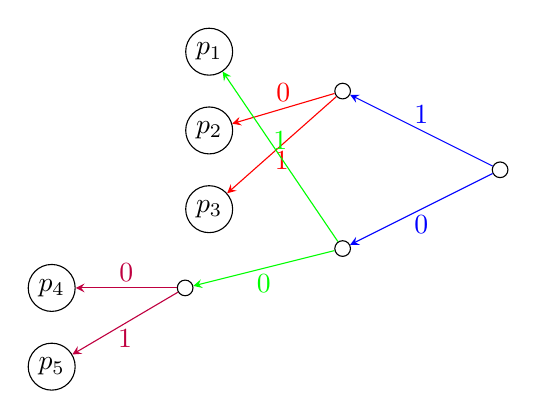
\begin{tikzpicture}[>=stealth, every node/.style={circle,draw,inner sep=2pt},
        level distance=1.5cm]
        % 根节点及各深度坐标
        \node[circle,draw] (root) at (0,0) {};
        \node[circle,draw] (u)    at (-2,1) {};   % 深度1 上
        \node[circle,draw] (l)    at (-2,-1){};   % 深度1 下
        \node[circle,draw] (l2)   at (-4,-1.5){}; % 深度2 右分支
        % 叶子节点:深度2的三个叶子和深度3的两个叶子
        \node[right] (p1) at (-4,1.5) {$p_1$};
        \node[right] (p2) at (-4,0.5) {$p_2$};
        \node[right] (p3) at (-4,-0.5) {$p_3$};
        \node[right] (p4) at (-6,-1.5) {$p_4$};
        \node[right] (p5) at (-6,-2.5) {$p_5$};
        % 定义标签样式,去掉圆圈和边框
        \tikzset{edgelabel/.style={inner sep=1pt,draw=none}}
        % 各树枝及标记
        \draw[->,blue]    (root) -- node[midway,above,edgelabel] {1} (u);
        \draw[->,blue]   (root) -- node[midway,below,edgelabel] {0} (l);
        \draw[->,red]    (u) -- node[midway,above,edgelabel] {0} (p2);
        \draw[->,red]    (u) -- node[midway,below,edgelabel] {1} (p3);
        \draw[->,green]  (l) -- node[midway,above,edgelabel] {1} (p1);
        \draw[->,green]  (l) -- node[midway,below,edgelabel] {0} (l2);
        \draw[->,purple] (l2) -- node[midway,above,edgelabel] {0} (p4);
        \draw[->,purple] (l2) -- node[midway,below,edgelabel] {1} (p5);
    \end{tikzpicture}
\end{center}
\end{example}

赫夫曼码是一种最优即时码。最优即时码是在期望长度最小意义下的即时码,它不是唯一的。

\begin{lemma}[最优即时码的刻画]
    任给分布$\mathbf{p}$,D=2,最优即时码必然满足:\\
    (1)$p_i>p_j\implies l_i\leq l_j$,即码长与概率反序;\\
    (2)最长的两个码字拥有相同的长度,且对应两个最小可能字符。

    此外,总能构造编码满足下述条件:\\
    (3)最长的两个码字仅在最后一位有差别

    称满足(3)的最优编码是典则的(canonical).
\end{lemma}
\begin{proof}
    (1)对$p_i>p_j$,设编码$C$满足$l_i\leq l_j$,$C'$为C交换i,j编码所得,则有
    \begin{align*}
        L(C')-L(C)&=p_j l_i+p_i l_j-p_i l_i-p_j l_j\\
        &=(p_j-p_i)(l_i-l_j)\geq 0
    \end{align*}

    (2)(3)两个最长码字在编码树中对应兄弟节点,否则必然可以修剪编码树(删除码字最后一位)。
\end{proof}

\begin{remark}
    (1)赫夫曼码满足
    \[H(X)\leq L(C)<H(X)+1\]
    (2)赫夫曼码是贪心算法,即局部最优$\to$全局最优
\end{remark}

\section{其他编码}

1.\textbf{香农码}

前面已经介绍。对于单个字符,赫夫曼码与香农码都可能有更短的码字长度,但平均意义下赫夫曼码才是最优编码。

香农码具有唯一竞争最优性:在单局游戏中,以甲、乙对同一随机序列的编码长短决定胜负,则香农码是一个很好的策略。

以下设D=2.
\begin{theorem}
    (1)设C为香农码,C'为其他唯一可译码,则
    \begin{align*}
        P\{l(X)\geq l'(X)+c\}\leq\frac{1}{2^{c-1}}
    \end{align*}

    (2)(香农码的唯一竞争最优性)设$p(x)$是二进制的,$l(x)=\log\dfrac{1}{p(x)}$为香农码的码字长度,则
    \begin{align*}
        \forall C',P\{l(X)<l'(X)\}\geq P\{l(X)>l'(X)\}
    \end{align*}
    取等$\iff \forall x,l(x)=l'(x)$。
\end{theorem}
\begin{corollary}
    对于非二进制的p(x),有\begin{align*}
        \mathbb{E} sgn(l(X)-l'(X)-1)\leq 0
    \end{align*}
    其中l为香农码C的码字长度。
\end{corollary}

2.\textbf{费纳(Fano)编码}

将概率值递减排列,然后选取k使得
\[\left|\sum_{i=1}^k p_i-\sum_{i=k+1}^m p_i\right|\]
最小(\textbf{二分概率}),概率高者赋0,概率低者赋1,再对子字符集重复此过程,直到每一字符分得唯一码字。

一般来说,这种编码不是最优编码,但是可以达到$L(C)\leq H(X)+2$.

3.\textbf{Shannon-Fano-Elias编码}

考虑累积分布函数$F(x)=\sum_{a\leq x}p(a)$及其修正$\overline{F}(x)$,$\overline{F}(x)$在间断点处取左右平均值。

以$\overline{F}(x)$的二进制表示的小数部分作为字符x的码字。在码字无限时,取前$\left\lceil \log\dfrac{1}{p(x)}\right\rceil+1$位即可。

编码的唯一性:以$\lfloor \overline{F}(x)\rfloor_{l(x)}$记$\overline{F}(x)$保留$l(x)$位。取$l(x)=\left\lceil \log\dfrac{1}{p(x)}\right\rceil+1$,则
\begin{align*}
    F(x)-\lfloor \overline{F}(x)\rfloor_{l(x)}<\frac{1}{2^{l(x)}}<\frac{1}{2}2^{\log p(x)}=\frac{p(x)}{2}
\end{align*}
即$\lfloor \overline{F}(x)\rfloor_{l(x)}$在F(x)下方跳变幅度以内,对应了唯一的区间。

这种编码的特点是:应用广泛;$L(C)<H(X)+2$;必为前缀码(考虑区间树可证)

\chapter{信道容量}

\section{通信系统模型}

\begin{definition}[信源模型]
    (1)根据信源输出信号所对应的随机过程是否平稳,分为稳恒(平稳)信源和非稳恒(非平稳)信源

    (2)根据特殊的随机过程类型,分为高斯信源、Markov信源等

    (3)信源字母表离散,信号取值时刻离散的稳恒信源称为离散稳恒信源
\end{definition}

\begin{definition}[信道模型]
    (1)按输入输出信号在幅值和时间上的取值分为离散信道(数字信道)、连续信道等\\
    离散信道(discrete channel)是至多可数的输入字母表$\mathcal{X}$和输出字母表$\mathcal{Y}$,及$\mathcal{X} $到$\mathcal{Y} $的转移概率模型构成的系统

    (2)如果信道输出值域信道在该时刻的输入有关,二与先前的输入输出等无关,则信道是无记忆信道(memoryless channel);否则为有记忆信道

    (3)按输入输出信号之间的关系是否确定,分为有噪信道和无噪信道等
\end{definition}

\begin{definition}[离散无记忆信道]
    离散无记忆信道(DMC)的转移概率模型可以用转移概率分布$p(y|x)$描述。
    
    设输入字母表为$\mathcal{X} $,输出字母表为$\mathcal{Y} $,该DMC可以用$$(\mathcal{X} ,p(x|y),\mathcal{Y} )$$表示
    
    离散无记忆信道的n次扩展可以用$$(\mathcal{X} ^n,p(x^n|y^n),\mathcal{Y} ^n)$$表示,其中
    \[p(y_k|x^k,y^{k-1})=p(y_k|x_k),\forall k\in\{1,2,\cdots,n\}\]

    进一步,如果信道不带反馈(如不明确指出,则默认不带反馈),即输入字符不依赖于过去的输出字符,即
    $$p(x_k|x^{k-1},y^{k-1})=p(x_k|x^{k-1}),\forall k$$
    则n次扩展的信道转移函数简化为
    \[p(y^k|x^k)=\prod_{i=1}^k p(y_i|x_i),\forall k\]
\end{definition}

\begin{definition}[信息信道容量]
    离散无记忆信道的信息信道容量(information channel capacity)定义为
    \[C = \max_{p(x)} I(X;Y)\]
\end{definition}
香农第二定理将指出信息信道容量=信道容量=信道最高码率=任意小误差传输比特数/信道使用次数。

$I(X;Y)$关于输入分布$p(x)$是紧集上的连续的凹函数,因此最大值存在且唯一,使用$\max$是合理的。

\begin{proposition}[信息信道容量的性质]
    \quad
    \begin{itemize}
        \item $C\geq 0$,取等$\iff$信道输出与输入独立
        \item $C\leq \log |\mathcal{X}|$,取等$\iff X,Y$独立且$X\sim U_{\mathcal{X} }$
        \item $C\leq \log |\mathcal{Y}|$,取等$\iff$存在输入分布使得输出分布为均匀分布
    \end{itemize}
\end{proposition}

\begin{definition}[对称信道]
    如果离散无记忆信道的概率转移矩阵$p(x|y)$是数独矩阵,则称该信道为对称信道(symmetric channel)。数独矩阵必然是双随机的。

    数独矩阵可以描述为:任何两行互为置换、任何两列也互为置换。
    
    如果每一行$p(\cdot|x)$都是同一分布的置换,且所有列的元素和$\sum_{x}p(y|x)$相同,则该信道是弱对称信道(weakly symmetric channel)
\end{definition}

\begin{theorem}
    对于弱对称信道,信息信道容量为
    \[C = \log |\mathcal{Y}| - H(p(\cdot|x))\]
    其中$p(\cdot|x)$为任一行的分布。取等$\iff$输入分布为均匀分布
\end{theorem}

\begin{example}[有噪打字机信道]
    该种信道的概率转移矩阵矩阵的基本特征是,对角线元素(不出错的概率)接近于1,除了对角线,每一行都有个别元素数值较大,而其他元素极小或为0。描述了考虑失误的打字机。

    输入、输出字母表相同,输入以0.5的概率被输出端无改变地接收,以0.5的概率变为下一个字母。字母表大小为26时,$C=13 bit/$传输:

    一方面,每次传输可以无误差地传输其中13个字符(仅传输奇数位置或偶数位置的字符);

    另一方面,$$C=\max I(X;Y)=\max [H(Y)-H(Y|X)]=\max H(Y)-1=\log 26-1=\log 13 bit/\text{传输}$$

    取等$\iff p(x)\sim U$
\end{example}

\begin{figure}[H]
    \centering
    \includegraphics[width=0.8\textwidth]{communicatioin_channel.jpg}
    \caption{离散通信信道模型}
\end{figure}

\begin{definition}[$(M,n)$码]
    信道$(\mathcal{X} ,p(y|x),\mathcal{Y} )$的$(M,n)$码由以下部分构成:\begin{itemize}
        \item 指标集$\{1,2,\cdots,M\}$
        \item 编码函数(encoding function)
        $$x^n:\{1,2,\cdots,M\}\to \mathcal{X} ^n$$
        生成码字(codewords)$x^n(1),x^n(2),\cdots,x^n(M)$,所有码字的集合称为码本(code-book)$$\mathcal{C}=\{x^n(1),x^n(2),\cdots,x^n(M)\}=\{\mathbf{x}_1,\mathbf{x}_2,\cdots,\mathbf{x}_M\}$$
        \item 译码函数
        $$g:\mathcal{Y} ^n\to\{1,2,\cdots,M\}$$
    \end{itemize}
\end{definition}

\begin{definition}[条件误差概率]
    已知指标$i$被发送,(给定发送符号时的)条件误差概率(conditional probability of error)为
    \[\lambda_i=P\{g(Y^n)\neq i|X^n=x^n(i)\}\]
    它衡量了特定符号在传输过程中的脆弱性或抗干扰能力。

    已知接收到符号y,(给定接收符号时的)条件误差概率为
    \[1-\max_{x}P\{X=x|Y=y\}\]
    反映了收到特定y后,接收端对这次判决的不确定性。条件误差概率通常指前者。
\end{definition}

\begin{definition}
    $(M,n)$码的最大误差概率(maximun probability of error)为
    \[\lambda^{(n)}=\max_{i\in\{1,2,\cdots,M\}} \lambda_i\]

    (算数)平均误差概率(average probability of error)为
    \[P^{(n)}_e=\overline{\lambda}=\frac{1}{M}\sum_{i=1}^{M}\lambda_i\]
\end{definition}

\begin{remark}
    如果指标W的选取服从均匀分布,则$P^{(n)}_e=P\{W\neq g(Y^n)\}$。
\end{remark}
\begin{remark}
    显然,$P_e^{(n)}\leq \lambda^{(n)}$。理应希望这二者差异大,但将证明:在相同码率下,平均误差概率小$\implies$最大误差概率小
\end{remark}

\begin{definition}[码率]
    $(M,n)$码的码率(rate)为
    \[R=\frac{\log M}{n}(bit/\text{传输})\]
    如果存在一个$(\lceil 2^{nR}\rceil,n)$码,满足$\lambda^{(n)}\to 0,n\to 0$,则称码率R是可达的(achievable)。一般将此编码简记为$(2^{nR},n)$。

    信道容量定义为可达码率的上确界。
\end{definition}

\begin{definition}[联合典型序列]
    服从分布$p(x,y)$的联合典型序列(jointly typical sequence)$\{(x^n,y^n)\}$所构成的集合$A^{(n)}_{\epsilon}$是指其经验熵与真实熵以$\epsilon$为界靠近的n长序列构成的集合,即:
    \begin{align*}
        A^{(n)}_{\epsilon}=\left\{(x^n,y^n)\in \mathcal{X}^n\times \mathcal{Y}^n:\right.
        &\left|-\frac{1}{n}\log p(x^n)-H(X)\right|<\epsilon,\\
        &\left|-\frac{1}{n}\log p(y^n)-H(Y)\right|<\epsilon,\\
        &\left.\left|-\frac{1}{n}\log p(x^n,y^n)-H(X,Y)\right|<\epsilon\right\}
    \end{align*}
    其中
    \[p(x^n,y^n)=\prod_{i=1}^{n}p(x_i,y_i)\]
\end{definition}

\begin{theorem}[联合AEP]
    设$(X^n,Y^n)$为服从$p(x^n,y^n)=\prod_{i=1}^n p(x_i,y_i)$的i.i.d.的n长序列,则

    \ding{172}$P\{(X^n,Y^n)\in A^{(n)}_{\epsilon}\}\to 1,n\to\infty$

    \ding{173}$|A^{(n)}_{\epsilon}|\leq 2^{n(H(X,Y)+\epsilon)}$

    \ding{174}如果$(\tilde{X}^n,\tilde{Y}^n)\sim p(x^n)p(y^n)$(i.e.$\tilde{X}^n$与$\tilde{Y}^n$独立且具有$p(x^n,y^n)$的边界分布,与$X^n,Y^n$分别同分布),则
    \begin{align*}
        P\left\{\left(\tilde{X}^n,\tilde{Y}^n\right)\in A^{(n)}_{\epsilon}\right\}\leq 2^{-n(I(X;Y)-3\epsilon)}
    \end{align*}
    且对于充分大的n,有\begin{align*}
        P\left\{\left(\tilde{X}^n,\tilde{Y}^n\right)\in A^{(n)}_{\epsilon}\right\}\geq (1-\epsilon)2^{-n(I(X;Y)+3\epsilon)}
    \end{align*}
\end{theorem}
\begin{proof}
    \ding{172}由弱大数定律,\begin{align*}
        &-\frac{1}{n}\log p(X^n)\to -\mathbb{E} \log p(X)=H(X)&\text{依概率}
    \end{align*}
    故$\forall \epsilon>0,\exists n_1,n>n_1$时,有\begin{align*}
        P\left\{\left|-\frac{1}{n}\log p(X^n)-H(X)\right|\geq \epsilon\right\}<\frac{\epsilon}{3}
    \end{align*}
    同理,\begin{align*}
        &-\frac{1}{n}\log p(Y^n)\to -\mathbb{E} \log p(Y)=H(Y)&\text{依概率}
    \end{align*}\begin{align*}
        &-\frac{1}{n}\log p(X^n,Y^n)\to -\mathbb{E} \log p(X,Y)=H(X,Y)&\text{依概率}
    \end{align*}
    从而有$n_2,n_3$,\begin{align*}
        n>n_2\implies P\left\{\left|-\frac{1}{n}\log p(Y^n)-H(Y)\right|\geq \epsilon\right\}<\frac{\epsilon}{3}
    \end{align*}\begin{align*}
        n>n_3\implies P\left\{\left|-\frac{1}{n}\log p(X^n,Y^n)-H(X,Y)\right|\geq \epsilon\right\}<\frac{\epsilon}{3}
    \end{align*}
    
    取$n>\max\{n_1,n_2,n_3\}$,则
    \begin{align*}
        P\{(X^n,Y^n)\in A^{(n)}_{\epsilon}\}>1-\epsilon
    \end{align*}

    \ding{173}注意到\begin{align*}
        1&=\sum p(x^n,y^n)\\
        &\geq \sum_{A^{(n)}_{\epsilon}}p(x^n,y^n)\\
        &\geq |A^{(n)}_{\epsilon}|\cdot 2^{-n(H(X<Y)+\epsilon)}
    \end{align*}
    这与要证的式子是等价的。最后一行成立是因为,根据$A^{(n)}_{\epsilon}$的定义(最后一条),每个$A^{(n)}_{\epsilon}$的元素$(x^n,y^n)$都满足\begin{align*}
        -n(H(X,Y)+\epsilon)<\log p(x^n,y^n)<-n(H(X,Y)-\epsilon)
    \end{align*}
    
    \ding{174}在这种假设下,有\begin{align*}
        P\left\{\left(\tilde{X}^n,\tilde{Y}^n\right)\in A^{(n)}_{\epsilon}\right\}&=\sum_{(x^n,y^n)\in A^{(n)}_{\epsilon}}p(x^n)p(y^n)\\
        &\leq 2^{n(H(X,Y)+\epsilon)}\cdot 2^{-n(H(X)-\epsilon)}\cdot 2^{-n(H(Y)-\epsilon)}\\
        &=2^{-n(I(X;Y)-3\epsilon)}
    \end{align*}

    在n充分大时,$P\left\{\left(\tilde{X}^n,\tilde{Y}^n\right)\in A^{(n)}_{\epsilon}\right\}\geq 1-\epsilon$,因此\begin{align*}
        1-\epsilon&\leq\sum_{(x^n,y^n)\in A^{(n)}_{\epsilon}}p(x^n,y^n)\\
        &\leq |A^{(n)}_{\epsilon}|\cdot 2^{-n(H(X,Y)-\epsilon)}
    \end{align*}
    即证后一不等式。
\end{proof}

\chapter{最后一页}

\end{document}